% Options for packages loaded elsewhere
\PassOptionsToPackage{unicode}{hyperref}
\PassOptionsToPackage{hyphens}{url}
%
\documentclass[
  ignorenonframetext,
]{beamer}
\usepackage{pgfpages}
\setbeamertemplate{caption}[numbered]
\setbeamertemplate{caption label separator}{: }
\setbeamercolor{caption name}{fg=normal text.fg}
\beamertemplatenavigationsymbolsempty
% Prevent slide breaks in the middle of a paragraph
\widowpenalties 1 10000
\raggedbottom
\setbeamertemplate{part page}{
  \centering
  \begin{beamercolorbox}[sep=16pt,center]{part title}
    \usebeamerfont{part title}\insertpart\par
  \end{beamercolorbox}
}
\setbeamertemplate{section page}{
  \centering
  \begin{beamercolorbox}[sep=12pt,center]{part title}
    \usebeamerfont{section title}\insertsection\par
  \end{beamercolorbox}
}
\setbeamertemplate{subsection page}{
  \centering
  \begin{beamercolorbox}[sep=8pt,center]{part title}
    \usebeamerfont{subsection title}\insertsubsection\par
  \end{beamercolorbox}
}
\AtBeginPart{
  \frame{\partpage}
}
\AtBeginSection{
  \ifbibliography
  \else
    \frame{\sectionpage}
  \fi
}
\AtBeginSubsection{
  \frame{\subsectionpage}
}
\usepackage{lmodern}
\usepackage{amssymb,amsmath}
\usepackage{ifxetex,ifluatex}
\ifnum 0\ifxetex 1\fi\ifluatex 1\fi=0 % if pdftex
  \usepackage[T1]{fontenc}
  \usepackage[utf8]{inputenc}
  \usepackage{textcomp} % provide euro and other symbols
\else % if luatex or xetex
  \usepackage{unicode-math}
  \defaultfontfeatures{Scale=MatchLowercase}
  \defaultfontfeatures[\rmfamily]{Ligatures=TeX,Scale=1}
\fi
\usetheme[]{Marburg}
\usefonttheme{structurebold}
% Use upquote if available, for straight quotes in verbatim environments
\IfFileExists{upquote.sty}{\usepackage{upquote}}{}
\IfFileExists{microtype.sty}{% use microtype if available
  \usepackage[]{microtype}
  \UseMicrotypeSet[protrusion]{basicmath} % disable protrusion for tt fonts
}{}
\makeatletter
\@ifundefined{KOMAClassName}{% if non-KOMA class
  \IfFileExists{parskip.sty}{%
    \usepackage{parskip}
  }{% else
    \setlength{\parindent}{0pt}
    \setlength{\parskip}{6pt plus 2pt minus 1pt}}
}{% if KOMA class
  \KOMAoptions{parskip=half}}
\makeatother
\usepackage{xcolor}
\IfFileExists{xurl.sty}{\usepackage{xurl}}{} % add URL line breaks if available
\IfFileExists{bookmark.sty}{\usepackage{bookmark}}{\usepackage{hyperref}}
\hypersetup{
  pdftitle={Estadística Inferencial},
  pdfauthor={Jackson M'coy Romero Plasencia},
  hidelinks,
  pdfcreator={LaTeX via pandoc}}
\urlstyle{same} % disable monospaced font for URLs
\newif\ifbibliography
\usepackage{color}
\usepackage{fancyvrb}
\newcommand{\VerbBar}{|}
\newcommand{\VERB}{\Verb[commandchars=\\\{\}]}
\DefineVerbatimEnvironment{Highlighting}{Verbatim}{commandchars=\\\{\}}
% Add ',fontsize=\small' for more characters per line
\usepackage{framed}
\definecolor{shadecolor}{RGB}{248,248,248}
\newenvironment{Shaded}{\begin{snugshade}}{\end{snugshade}}
\newcommand{\AlertTok}[1]{\textcolor[rgb]{0.94,0.16,0.16}{#1}}
\newcommand{\AnnotationTok}[1]{\textcolor[rgb]{0.56,0.35,0.01}{\textbf{\textit{#1}}}}
\newcommand{\AttributeTok}[1]{\textcolor[rgb]{0.77,0.63,0.00}{#1}}
\newcommand{\BaseNTok}[1]{\textcolor[rgb]{0.00,0.00,0.81}{#1}}
\newcommand{\BuiltInTok}[1]{#1}
\newcommand{\CharTok}[1]{\textcolor[rgb]{0.31,0.60,0.02}{#1}}
\newcommand{\CommentTok}[1]{\textcolor[rgb]{0.56,0.35,0.01}{\textit{#1}}}
\newcommand{\CommentVarTok}[1]{\textcolor[rgb]{0.56,0.35,0.01}{\textbf{\textit{#1}}}}
\newcommand{\ConstantTok}[1]{\textcolor[rgb]{0.00,0.00,0.00}{#1}}
\newcommand{\ControlFlowTok}[1]{\textcolor[rgb]{0.13,0.29,0.53}{\textbf{#1}}}
\newcommand{\DataTypeTok}[1]{\textcolor[rgb]{0.13,0.29,0.53}{#1}}
\newcommand{\DecValTok}[1]{\textcolor[rgb]{0.00,0.00,0.81}{#1}}
\newcommand{\DocumentationTok}[1]{\textcolor[rgb]{0.56,0.35,0.01}{\textbf{\textit{#1}}}}
\newcommand{\ErrorTok}[1]{\textcolor[rgb]{0.64,0.00,0.00}{\textbf{#1}}}
\newcommand{\ExtensionTok}[1]{#1}
\newcommand{\FloatTok}[1]{\textcolor[rgb]{0.00,0.00,0.81}{#1}}
\newcommand{\FunctionTok}[1]{\textcolor[rgb]{0.00,0.00,0.00}{#1}}
\newcommand{\ImportTok}[1]{#1}
\newcommand{\InformationTok}[1]{\textcolor[rgb]{0.56,0.35,0.01}{\textbf{\textit{#1}}}}
\newcommand{\KeywordTok}[1]{\textcolor[rgb]{0.13,0.29,0.53}{\textbf{#1}}}
\newcommand{\NormalTok}[1]{#1}
\newcommand{\OperatorTok}[1]{\textcolor[rgb]{0.81,0.36,0.00}{\textbf{#1}}}
\newcommand{\OtherTok}[1]{\textcolor[rgb]{0.56,0.35,0.01}{#1}}
\newcommand{\PreprocessorTok}[1]{\textcolor[rgb]{0.56,0.35,0.01}{\textit{#1}}}
\newcommand{\RegionMarkerTok}[1]{#1}
\newcommand{\SpecialCharTok}[1]{\textcolor[rgb]{0.00,0.00,0.00}{#1}}
\newcommand{\SpecialStringTok}[1]{\textcolor[rgb]{0.31,0.60,0.02}{#1}}
\newcommand{\StringTok}[1]{\textcolor[rgb]{0.31,0.60,0.02}{#1}}
\newcommand{\VariableTok}[1]{\textcolor[rgb]{0.00,0.00,0.00}{#1}}
\newcommand{\VerbatimStringTok}[1]{\textcolor[rgb]{0.31,0.60,0.02}{#1}}
\newcommand{\WarningTok}[1]{\textcolor[rgb]{0.56,0.35,0.01}{\textbf{\textit{#1}}}}
\usepackage{graphicx,grffile}
\makeatletter
\def\maxwidth{\ifdim\Gin@nat@width>\linewidth\linewidth\else\Gin@nat@width\fi}
\def\maxheight{\ifdim\Gin@nat@height>\textheight\textheight\else\Gin@nat@height\fi}
\makeatother
% Scale images if necessary, so that they will not overflow the page
% margins by default, and it is still possible to overwrite the defaults
% using explicit options in \includegraphics[width, height, ...]{}
\setkeys{Gin}{width=\maxwidth,height=\maxheight,keepaspectratio}
% Set default figure placement to htbp
\makeatletter
\def\fps@figure{htbp}
\makeatother
\setlength{\emergencystretch}{3em} % prevent overfull lines
\providecommand{\tightlist}{%
  \setlength{\itemsep}{0pt}\setlength{\parskip}{0pt}}
\setcounter{secnumdepth}{-\maxdimen} % remove section numbering
\usepackage{ragged2e}
\usepackage{color}
\usepackage{listings}
\AtBeginSubsection{}

\title{Estadística Inferencial}
\author{Jackson M'coy Romero Plasencia}
\date{Ayacucho 2020}
\institute{\large Universidad Nacional de San Cristóbal de Huamanga \and \normalsize Departamento Académico de Matemática y Física}

\begin{document}
\frame{\titlepage}

\begin{frame}
  \tableofcontents[hideallsubsections]
\end{frame}
\hypertarget{distribuciones-de-probabilidad}{%
\section{Distribuciones de
Probabilidad}\label{distribuciones-de-probabilidad}}

\hypertarget{section}{%
\subsection{}\label{section}}

\hypertarget{distribuciones-de-probabilidad-en-r}{%
\subsection{Distribuciones de Probabilidad en
R}\label{distribuciones-de-probabilidad-en-r}}

\begin{frame}{Distribuciones de Probabilidad en R}

\justifying El paquete stats de R (que se instala por defecto al
instalar R, y se carga en memoria siempre que iniciamos sesión)
implementa numerosas funciones para la realización de cálculos asociados
a distintas distribuciones de probabilidad.

Para obtener una lista completa de las distribuciones disponibles en R
puede utilizar el siguiente comando: \color{blue}
help(``Distributions'')

\end{frame}

\hypertarget{argumentos-en-r}{%
\subsection{Argumentos en R}\label{argumentos-en-r}}

\begin{frame}{Argumentos en R}

\justifying Para cada distribución hay cuatro comandos. Los comandos
para cada distribución están precedidos de una letra para indicar la
funcionalidad:

\begin{itemize}
    \item  d: devuelve la función de densidad de probabilidad
    \item  p: devuelve la función de densidad acumulada
    \item q: devuelve la función de densidad acumulativa inversa (cuantiles)
    \item  r: devuelve los números generados aleatoriamente
 \end{itemize}

\end{frame}

\hypertarget{distribuciones-de-probabilidad-discretas}{%
\subsection{Distribuciones de Probabilidad
Discretas}\label{distribuciones-de-probabilidad-discretas}}

\hypertarget{distribucuxedon-binomal-binnp}{%
\subsection{\texorpdfstring{Distribucíon Binomal
\(Bin(n,p)\)}{Distribucíon Binomal Bin(n,p)}}\label{distribucuxedon-binomal-binnp}}

\begin{frame}{Distribucíon Binomal \(Bin(n,p)\)}

\justifying Es una distribución de probabilidad discreta; su función de
cuantía o de masa de probabilidad está dada por:
\[f_x{(x,n,p)}=f_x (x)=P(X=x)=\binom{n}{p}p^x (1-p)^{n-x} \quad x=\overline{0,n}\]
Donde:

\begin{itemize}
    \item n: \mbox{número de ensayos independientes}
    \item p y q: \mbox{probabilidad de éxitos y fracaso, p+q=1}
    \item x: \mbox{número de éxitos en n ensayos}
\end{itemize}

\end{frame}

\hypertarget{section-1}{%
\subsection{}\label{section-1}}

\begin{frame}[fragile]{}

\justifying Suponga que hay doce preguntas de opción múltiple en un
examen de matemáticas. Cada pregunta tiene cinco posibles respuestas, y
sólo una de ellas es correcta. Encuentre la probabilidad de tener cuatro
o menos respuestas correctas .\(P(X\leq 4)=?\)

\begin{Shaded}
\begin{Highlighting}[]
\NormalTok{n=}\DecValTok{12}
\NormalTok{p=}\DecValTok{1}\OperatorTok{/}\DecValTok{5}
\KeywordTok{pbinom}\NormalTok{(}\DecValTok{4}\NormalTok{,}\DataTypeTok{size=}\NormalTok{n,}\DataTypeTok{prob=}\NormalTok{p)}
\end{Highlighting}
\end{Shaded}

\begin{verbatim}
## [1] 0.9274445
\end{verbatim}

\begin{Shaded}
\begin{Highlighting}[]
\NormalTok{n=}\DecValTok{12}
\NormalTok{p=}\DecValTok{1}\OperatorTok{/}\DecValTok{5}
\KeywordTok{round}\NormalTok{(}\KeywordTok{dbinom}\NormalTok{(}\DecValTok{0}\OperatorTok{:}\DecValTok{4}\NormalTok{,}\DataTypeTok{size=}\NormalTok{n,}\DataTypeTok{prob=}\NormalTok{p),}\DecValTok{3}\NormalTok{)}
\end{Highlighting}
\end{Shaded}

\begin{verbatim}
## [1] 0.069 0.206 0.283 0.236 0.133
\end{verbatim}

\begin{Shaded}
\begin{Highlighting}[]
\KeywordTok{round}\NormalTok{(}\KeywordTok{sum}\NormalTok{(}\KeywordTok{dbinom}\NormalTok{(}\DecValTok{0}\OperatorTok{:}\DecValTok{4}\NormalTok{,}\DataTypeTok{size=}\NormalTok{n,}\DataTypeTok{prob=}\NormalTok{p)),}\DecValTok{3}\NormalTok{)}
\end{Highlighting}
\end{Shaded}

\begin{verbatim}
## [1] 0.927
\end{verbatim}

\end{frame}

\hypertarget{distribuciuxf3n-poisson-plambda}{%
\subsection{\texorpdfstring{Distribución Poisson
\(P(\lambda)\)}{Distribución Poisson P(\textbackslash lambda)}}\label{distribuciuxf3n-poisson-plambda}}

\begin{frame}{Distribución Poisson \(P(\lambda)\)}

La función de cuantía o masa de probabilidad es:

\[f_x(x,\lambda)=P(X=x)=\frac{e^{-\lambda\, }\lambda^x}{x!}\quad x=0,1,2,...\]
Donde:

\begin{itemize}
    \item X: número de éxitos por unidades de tiempo, espacio, área, etc.
    \item $\lambda$ número promedio de éxitos por unidades de tiempo, espacio, área, etc.
\end{itemize}

\end{frame}

\hypertarget{section-2}{%
\subsection{}\label{section-2}}

\begin{frame}[fragile]{}

\justifying Si hay doce coches cruzando un puente por minuto en
promedio, encuentre la probabilidad de tener diecisiete o más coches
cruzando el puente en un minuto en particular.

\[\begin{matrix}
P(X\geq 17) & = & 1 -P(X< 17)\\ 
 &  = &1 - P(X\leq  16) \\ 
 &  = &1- P(16,12) \\ 
 &  = & 0\mbox{.}101291
\end{matrix}\]

\begin{Shaded}
\begin{Highlighting}[]
\NormalTok{l=}\DecValTok{12}
\DecValTok{1}\OperatorTok{-}\KeywordTok{ppois}\NormalTok{(}\DecValTok{16}\NormalTok{,}\DataTypeTok{lambda =}\NormalTok{l)}
\end{Highlighting}
\end{Shaded}

\begin{verbatim}
## [1] 0.101291
\end{verbatim}

\end{frame}

\hypertarget{distrbuciuxf3n-de-probabilidad-continua}{%
\subsection{Distrbución de Probabilidad
Continua}\label{distrbuciuxf3n-de-probabilidad-continua}}

\hypertarget{distribuciuxf3n-normal-nmusigma}{%
\subsection{\texorpdfstring{Distribución Normal
\(N(\mu,\sigma)\)}{Distribución Normal N(\textbackslash mu,\textbackslash sigma)}}\label{distribuciuxf3n-normal-nmusigma}}

\begin{frame}{Distribución Normal \(N(\mu,\sigma)\)}

\justifying

La función de densidad de probabilidad de la distribución Normal es:

\[f_X (x,\mu,\sigma)=\displaystyle\frac{1}{\sqrt{2\pi}\, \sigma}e^{-\frac{(x-\mu)^2}{2\sigma^2}} \]
Donde:

\begin{itemize}
    \item $\mu$ es la media( mediana y moda)
    \item $\sigma$ desviación estándar $\sigma>0$
    \item El proceso para estandarizar la distribución Normal consiste en transformar la variable Normal  $N(\mu,\sigma)$  $N(0,1)$,es decir:
    $$Z=\frac{X-\mu}{\sigma} $$
\end{itemize}

\end{frame}

\hypertarget{section-3}{%
\subsection{}\label{section-3}}

\begin{frame}[fragile]{}

\justifying En una ciudad se estima que la temperatura máxima en el mes
de junio sigue una distribución normal, con media 23° y desviación
típica 5°. Calcular el número de días del mes en los que se espera
alcanzar máximas entre 21° y 27°. \[\begin{array}{rcl}
P(21 \leq X \leq 27) & = &\displaystyle P\Big( \frac{21-23}{5} \leq \frac{X-\mu}{\sigma} \leq  \frac{27-23}{5}\Big)\\ 
 &  = & \displaystyle P\Big( \frac{-2}{5} \leq Z \leq  \frac{4}{5}\Big) \\ 
 &  = & \displaystyle P\Big(-0.4 \leq Z \leq  0.8\Big) \\ 
 &  = & P(Z\leq 0.8)-P(Z\leq -0.4)
\end{array}\]

\begin{Shaded}
\begin{Highlighting}[]
\KeywordTok{pnorm}\NormalTok{(}\FloatTok{0.8}\NormalTok{)}\OperatorTok{-}\KeywordTok{pnorm}\NormalTok{(}\OperatorTok{-}\FloatTok{0.4}\NormalTok{)}\CommentTok{# Dist. Normal Estándar}
\end{Highlighting}
\end{Shaded}

\begin{verbatim}
## [1] 0.4435663
\end{verbatim}

\begin{Shaded}
\begin{Highlighting}[]
\KeywordTok{pnorm}\NormalTok{(}\DecValTok{27}\NormalTok{,}\DecValTok{23}\NormalTok{,}\DecValTok{5}\NormalTok{)}\OperatorTok{-}\KeywordTok{pnorm}\NormalTok{(}\DecValTok{21}\NormalTok{,}\DecValTok{23}\NormalTok{,}\DecValTok{5}\NormalTok{)}\CommentTok{#Dist. Normal General}
\end{Highlighting}
\end{Shaded}

\begin{verbatim}
## [1] 0.4435663
\end{verbatim}

\end{frame}

\hypertarget{section-4}{%
\subsection{}\label{section-4}}

\begin{frame}{}

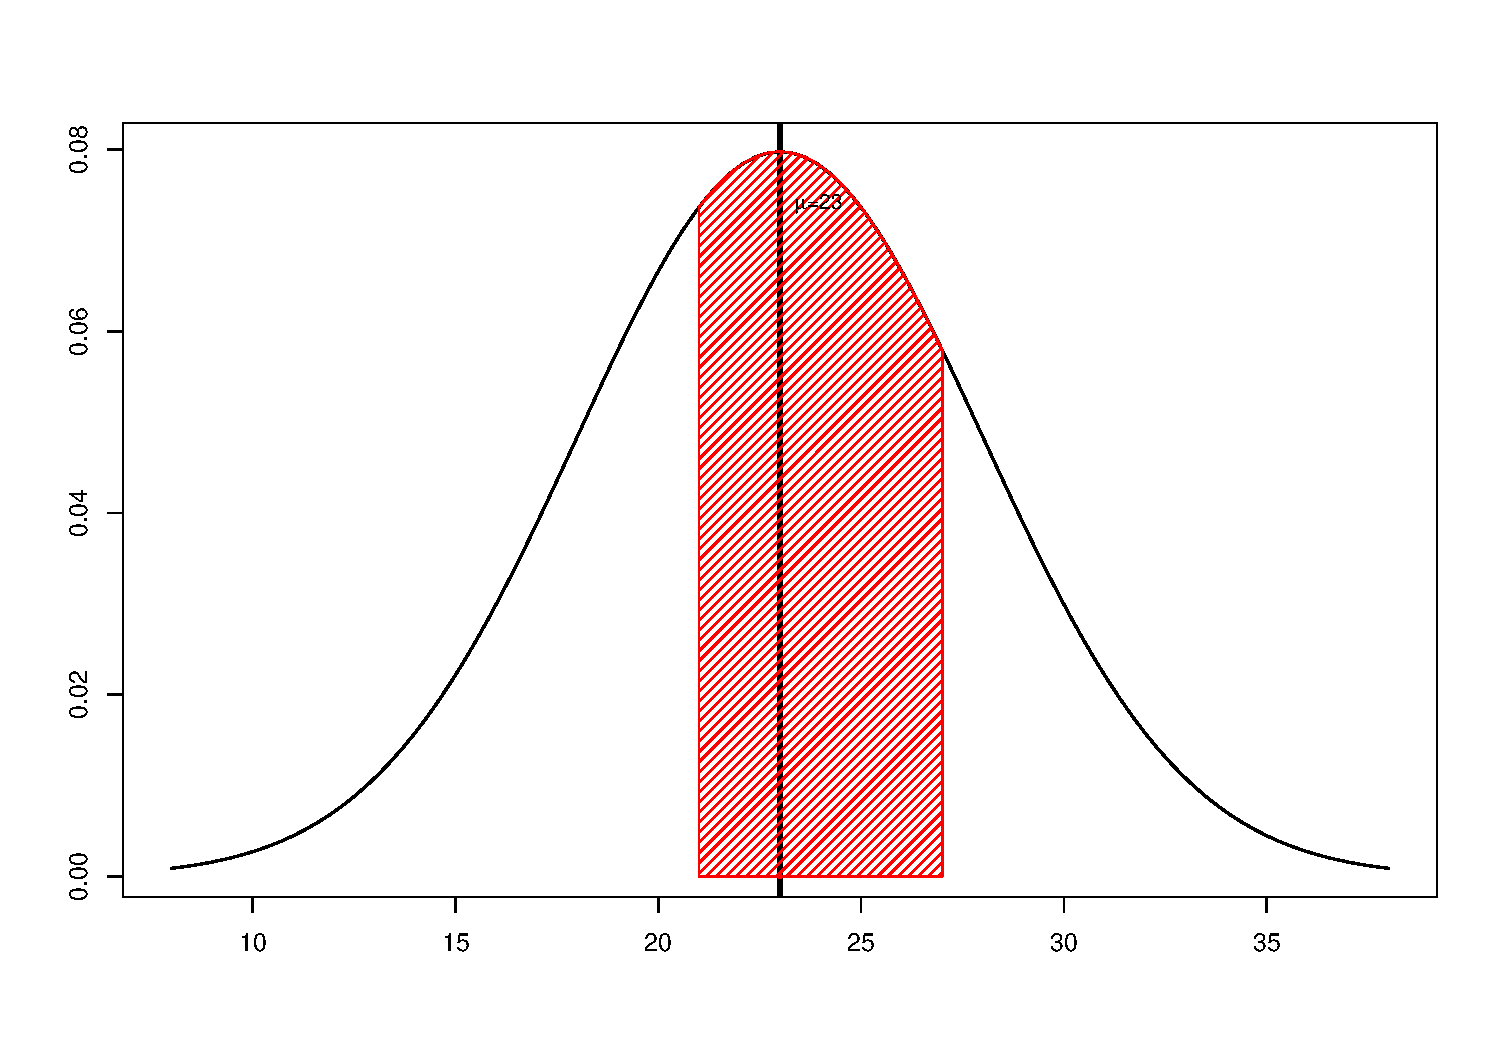
\includegraphics{clase1Inferencia_files/figure-beamer/unnamed-chunk-6-1.pdf}

\end{frame}

\hypertarget{distribuciuxf3n-chi-cuadrado-chi_n2}{%
\subsection{\texorpdfstring{Distribución Chi Cuadrado
\(\chi_{(n)}^{2}\)}{Distribución Chi Cuadrado \textbackslash chi\_\{(n)\}\^{}\{2\}}}\label{distribuciuxf3n-chi-cuadrado-chi_n2}}

\begin{frame}{Distribución Chi Cuadrado \(\chi_{(n)}^{2}\)}

\justifying Teorema: Sean \(X_1,X_2,...,X_n\) variables aleatorias
independientes e identicamente distribuídas segun la distribución
normal.

\[\sum_{i=1}^{n}\Bigg(\frac{X_i-\mu}{\sigma}\Bigg)^2 \longrightarrow \chi_{(n)}^{2} \]
cuya función de densidad,
\[f_X(x,n)=\displaystyle \frac{X^{n/2-1} \,\,e^{-x/2}}{2^{n/2}\,\,\Gamma(n/2)} \]

\[\begin{array}{rcl}
E(X) & = &n\\ 
 &   & \\ 
Var(X) &  = & 2n
\end{array}\]

\end{frame}

\hypertarget{distribuciuxf3n-t--student-t_n}{%
\subsection{\texorpdfstring{Distribución t- Student
\(t_{(n)}\)}{Distribución t- Student t\_\{(n)\}}}\label{distribuciuxf3n-t--student-t_n}}

\begin{frame}{Distribución t- Student \(t_{(n)}\)}

\justifying Teorema: Sea \(Z\) y \(V\) variables aleatorias
independientes distribuídas segun la distribución normal estándar y chi
cuadrado en v grados de libertad, respectivamente.

\[t=\frac{Z}{\sqrt{V/v}} \longrightarrow t_{(v)} \] cuya función de
densidad,
\[f_T(t,v)=\displaystyle \frac{\Gamma{(v+1)/2}}{\sqrt{v\pi} \,\,\Gamma(v/2)}(1+t^2/v)^{-(v+1)/2} \]

\[\begin{array}{rcl}
E(T) & = &0\\ 
 &   & \\ 
Var(T) &  = &\displaystyle \frac{v}{v-2} 
\end{array}\]

\end{frame}

\hypertarget{distribuciuxf3n-f--snedecor-f_mn}{%
\subsection{\texorpdfstring{Distribución F- Snedecor
\(F_{(m,n)}\)}{Distribución F- Snedecor F\_\{(m,n)\}}}\label{distribuciuxf3n-f--snedecor-f_mn}}

\begin{frame}{Distribución F- Snedecor \(F_{(m,n)}\)}

\justifying Teorema: Sea \(X\) y \(Y\) variables aleatorias
independientes distribuídas segun la distribución Chi cuadrado con m y n
grados de libertad, respectivamente.

\[\frac{X/m}{Y/n} \longrightarrow F_{(m,n)} \]

\[ E(F) =\displaystyle\frac{n}{n-2} \]

\end{frame}

\hypertarget{introducciuxf3n-a-la-inferencia-estaduxedstica}{%
\section{Introducción a la Inferencia
Estadística}\label{introducciuxf3n-a-la-inferencia-estaduxedstica}}

\hypertarget{definiciuxf3n-muestra-aleatoria}{%
\subsection{Definición: Muestra
Aleatoria}\label{definiciuxf3n-muestra-aleatoria}}

\begin{frame}{Definición: Muestra Aleatoria}

Una muestra aleatoria de tamaño \(n\) de una variable aleatorio \(X\) es
un conjunto de \(n\) - variables aleatorias \(X_1,X_2,...,X_n\), tal
que:

\begin{itemize}
  \item Todas $X_1,X_2,...,X_n \quad i=\overline{1,n}$ son independientes
  \item $X_1,X_2,...,X_n$ tienen la misma distribución, es decir:
        $$F_{X_i}(t)=F_{X}(t)\quad \forall \,\,i=\overline{1,n}$$
        $$\quad \longrightarrow f_{X_1,X_2,...,X_n}(x_1,x_2,...,x_n)=\prod_{i=1}^{n} f_{X_i}(x_i) $$
\end{itemize}

\end{frame}

\hypertarget{por-ejemplo}{%
\subsection{Por ejemplo:}\label{por-ejemplo}}

\begin{frame}{Por ejemplo:}

Sea \(X\) una variable aleatorio con distribución normal, se elije una
m.a de tamaño 2.

\[\begin{array}{rcl}
X_1: &  &E(X_1)=\mu \quad Var(X_1)=\sigma^2\\ 
 &   & \\ 
X_2: & &E(X_2)=\mu \quad Var(X_2)=\sigma^2\\ 
\end{array}\]

\justifying Sea \(X\) una variable aleatorio con distribución binomial
\(Bin(10,0.2)\), se elije una m.a de tamaño 2.

\[\begin{array}{rcl}
X_1: &  &E(X_1)=2 \quad Var(X_1)=1.6\\ 
 &   & \\ 
X_2: & &E(X_2)=2 \quad Var(X_2)=1.6\\ 
\end{array}\]

\end{frame}

\hypertarget{section-5}{%
\subsection{}\label{section-5}}

\begin{frame}{}

\justifying La vida útil( en miles de horas ) de una batería es una
variable aleatoria \(X\) con función de densidad:

\[f_X (x)=\left\{\begin{matrix}
 2-2x& 0\leq  x\leq 1\\ 
 & \\ 
 0& e.o.c 
\end{matrix}\right.
\]

En este caso, no hay información acerca de lo parámetros poblacionales(
\(E(X), Var(X)\)). Debemos realizar el cálculo de dichos parámetros y
luego ver las características de la muestra aleatoria

Vamos a estimar los parámetros a partir de simulaciones con el método
Monte Carlo.

\end{frame}

\hypertarget{section-6}{%
\subsection{}\label{section-6}}

\begin{frame}[fragile]{}

Simulación de Monte Carlo para integrales

\begin{Shaded}
\begin{Highlighting}[]
\NormalTok{ MC.simple.est <-}\StringTok{ }\ControlFlowTok{function}\NormalTok{(g, a, b, }\DataTypeTok{n=}\FloatTok{1e5}\NormalTok{) \{}
\NormalTok{   xi <-}\StringTok{ }\KeywordTok{runif}\NormalTok{(n,a,b)      }\CommentTok{# step 1}
\NormalTok{   g.mean <-}\StringTok{ }\KeywordTok{mean}\NormalTok{(}\KeywordTok{g}\NormalTok{(xi))   }\CommentTok{# step 2}
\NormalTok{   (b}\OperatorTok{-}\NormalTok{a)}\OperatorTok{*}\NormalTok{g.mean            }\CommentTok{# step 3}
\NormalTok{ \}}
\end{Highlighting}
\end{Shaded}

Simulación de Monte Carlo Valor Esperado

\begin{Shaded}
\begin{Highlighting}[]
\NormalTok{ mediap<-}\StringTok{ }\ControlFlowTok{function}\NormalTok{(g, a, b, }\DataTypeTok{n=}\FloatTok{1e5}\NormalTok{) \{}
\NormalTok{    xi <-}\StringTok{ }\KeywordTok{runif}\NormalTok{(n,a,b)      }\CommentTok{# step 1}
\NormalTok{    g.mean <-}\StringTok{ }\KeywordTok{mean}\NormalTok{(}\KeywordTok{g}\NormalTok{(xi)}\OperatorTok{*}\NormalTok{xi)}\CommentTok{# step 2}
\NormalTok{    (b}\OperatorTok{-}\NormalTok{a)}\OperatorTok{*}\NormalTok{g.mean            }\CommentTok{# step 3}
\NormalTok{ \}}
\end{Highlighting}
\end{Shaded}

\end{frame}

\hypertarget{section-7}{%
\subsection{}\label{section-7}}

\begin{frame}[fragile]{}

Simulación de Monte Carlo Varianza

\begin{Shaded}
\begin{Highlighting}[]
\NormalTok{varp<-}\ControlFlowTok{function}\NormalTok{(g, a, b, }\DataTypeTok{n=}\FloatTok{1e5}\NormalTok{) \{}
\NormalTok{    xi <-}\StringTok{ }\KeywordTok{runif}\NormalTok{(n,a,b)     }\CommentTok{# step 1}
\NormalTok{    g.mean <-}\StringTok{ }\KeywordTok{mean}\NormalTok{(}\KeywordTok{g}\NormalTok{(xi)}\OperatorTok{*}\NormalTok{xi}\OperatorTok{^}\DecValTok{2}\NormalTok{)}\OperatorTok{-}
\StringTok{      }\NormalTok{(}\KeywordTok{mean}\NormalTok{(}\KeywordTok{g}\NormalTok{(xi)}\OperatorTok{*}\NormalTok{xi))}\OperatorTok{^}\DecValTok{2}   \CommentTok{# step 2}
\NormalTok{    (b}\OperatorTok{-}\NormalTok{a)}\OperatorTok{*}\NormalTok{g.mean\}          }\CommentTok{# step 3}
\end{Highlighting}
\end{Shaded}

\begin{Shaded}
\begin{Highlighting}[]
\NormalTok{ g <-}\StringTok{ }\ControlFlowTok{function}\NormalTok{(x) }\DecValTok{2-2}\OperatorTok{*}\NormalTok{x}
 \KeywordTok{MC.simple.est}\NormalTok{(g, }\DecValTok{0}\NormalTok{, }\DecValTok{1}\NormalTok{)}
\end{Highlighting}
\end{Shaded}

\begin{verbatim}
## [1] 0.9981907
\end{verbatim}

\begin{Shaded}
\begin{Highlighting}[]
 \KeywordTok{mediap}\NormalTok{(g,}\DecValTok{0}\NormalTok{,}\DecValTok{1}\NormalTok{)}
\end{Highlighting}
\end{Shaded}

\begin{verbatim}
## [1] 0.3333036
\end{verbatim}

\begin{Shaded}
\begin{Highlighting}[]
 \KeywordTok{varp}\NormalTok{(g,}\DecValTok{0}\NormalTok{,}\DecValTok{1}\NormalTok{)}
\end{Highlighting}
\end{Shaded}

\begin{verbatim}
## [1] 0.05581654
\end{verbatim}

\end{frame}

\hypertarget{definiuxf3n-estaduxedstica-o-estimador}{%
\subsection{Definión: Estadística o
estimador}\label{definiuxf3n-estaduxedstica-o-estimador}}

\begin{frame}{Definión: Estadística o estimador}

Se denomina estadística a cualquier función de las variables aleatorias
que constituyen la muestra.

\justifying Una estadística es una variablea aleatoria
\(Y=H(X_1,X_2,...,X_n)\), cuyo valor es un número real
\(y=H(x_1,x_2,...,x_n)\)

Algunas estadísticas importantes sus valores calculados a partir de la
muestra aleatoria:

\[\overline{X}=\frac{1}{n} \sum_{i=1}^{n}X_i\,\,(\mbox{Variable aleatoria})\quad  \overline{x}=\frac{1}{n} \sum_{i=1}^{n}x_i\,\,(\mbox{valor})\]
\[S^2=\frac{1}{n} \sum_{i=1}^{n}(X_i-\overline{X})^2\,\,(\mbox{con valor})\quad  s^2=\frac{1}{n} \sum_{i=1}^{n}(x_i-\overline{x})^2\]

\end{frame}

\hypertarget{section-8}{%
\subsection{}\label{section-8}}

\begin{frame}{}

\[\overline{X}=\frac{1}{n} \sum_{i=1}^{n}X_i \longrightarrow N(\mu, \displaystyle \frac{\sigma^2}{n} ) \]

\end{frame}

\hypertarget{section-9}{%
\subsection{}\label{section-9}}

\begin{frame}{}

\[P(|X-\mu|\leq 2\sigma)=0.9544\] \[P(|X-\mu|\leq \sigma)=0.68\]
\[P(|X-\mu|\leq 3\sigma)=0.9544\]

\end{frame}

\end{document}
